\section{Iris}\label{sec:Iris}

Um dos datasets que o grupo escolheu foi o Iris. Este é, segundo os autores, o maior conjunto de dados conhecido disponível para ser aplicado em processos de extração de conhecimento. O conjunto de dados contém 3 classes com 50 instâncias cada uma, onde cada classe refere-se a um tipo de planta de Íris. Uma classe é linearmente separável dos outros 2 e estes não são linearmente separáveis uns dos outros.

\subsection{Objetivos do estudo}

Uma das razões pelas quais o grupo escolheu este dataset foi o grande número e variedade de artigos científicos publicados de estudos que o utilizaram. Com o estudo deste conjunto de dados e, como o autor refere, pretende-se descobrir a relações entre os diferentes atributos tendo em vista a previsão da classe de Íris, dentro das que existem dados. Seguindo as recomendações do autor do dataset esse foi o nosso grande foco para este estudo.


\subsection{Atributos do conjunto de dados}

De seguida listam-se os atributos originais do conjunto de dados e a sua descrição.

\begin{table}[]
\centering
\resizebox{\textwidth}{!}{\begin{tabular}{|l|l|l|}
\hline
Atributo     & Descrição                                               & Tipo                            \\ \hline
Sepal Length & Comprimento da sépala (peça constituinte da flor) em cm & Numérico                        \\ \hline
Sepal Width  & Largura da sépala (peça constituinte da flor) em cm     & Numérico                        \\ \hline
Petal Length & Comprimento da pétala em cm                             & Numérico                        \\ \hline
Petal Width  & Largura da pétala em cm                                 & Numérico                        \\ \hline
Class        & Tipo de Íris (Setosa, Versicolour ou Virginica)         & Set.,Vers. ou Virg. \\ \hline
\end{tabular}}
\end{table}

Pela análise aos atributos conseguimos perceber que o atributo classe é aquele a prever pelo cálculo dos restantes e que o domínio dos atributos é bastante simples.

\subsection{Preparação do conjunto}


Como já foi anteriormente referido houve alguns aspetos que nos chamaram atenção para este conjunto de dados, sendo um deles o facto de os dados estarem bem recolhidos. O primeiro passo para a preparação do conjunto foi verificar se existiriam diferentes fontes de dados para fazer a integração/uniformização dos dados, tal não foi necessário já que se verificou que apenas existia uma fonte de dados.
O passo seguinte foi verificar a existência de atributos redundantes, chegando à conclusão que não existem. Ficou apenas a nota de que o atributo classe seria um atributo a prever e não deveria ser considerado como dado de \"entrada\".
Após estes dois passos prosseguimos para a discretização de todos os atributos, exceto a Class. 

\begin{figure}[H]
    \centering
    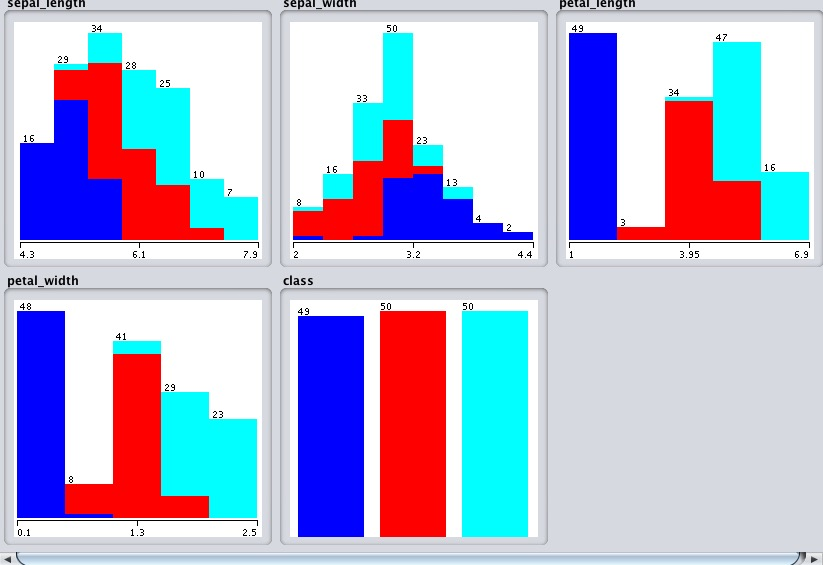
\includegraphics[scale=0.4]{tex/img/img2i.jpg}
    \caption{Gráfico dos dados antes da discretização}
    \label{fig:antes}
\end{figure}

\begin{figure}[H]
    \centering
    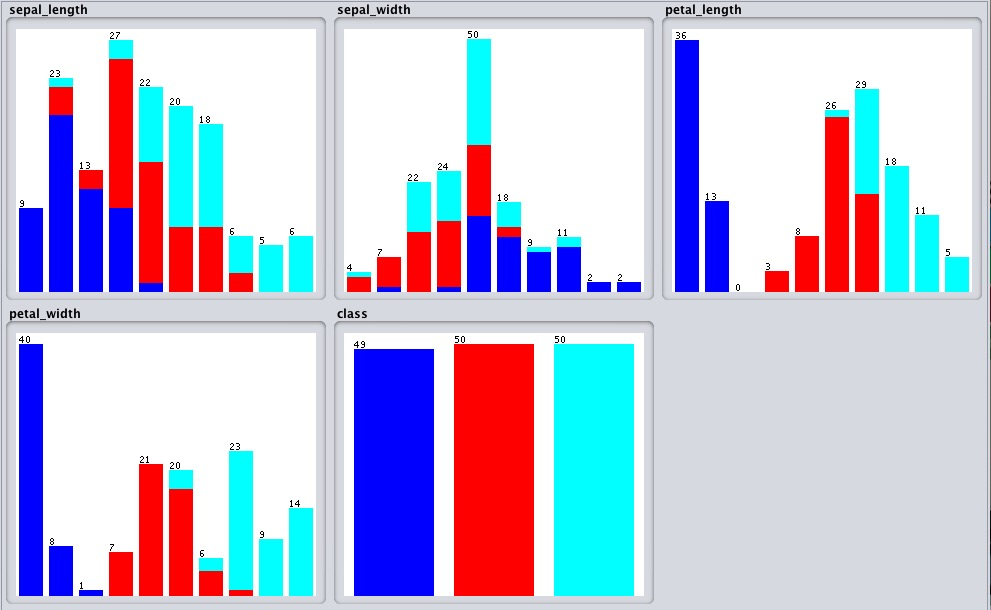
\includegraphics[scale=0.3]{tex/img/img1i.jpg}
    \caption{Gráfico dos dados após discretização}
    \label{fig:apos}
\end{figure}

\newpage
\subsection{Classificação}

\textbf{Algoritmo J48}

O primeiro Algoritmo de Classificação aplicado foi o J48, com a finalidade de construir uma árvore de decisão baseada no conjunto de dados. O algoritmo foi aplicado duas vezes uma delas usando o conjunto de dados como conjunto de treino com uma média absoluta de erro de 2\% e utilizando \"cross-validation\" com uma média absoluta de erro de 3\%. Preferimos então continuar a usar o conjunto como conjunto de treino.

\begin{lstlisting}[breaklines,frame=single]

=== Classifier model (full training set) ===

J48 pruned tree
------------------

petal_width <= 0.6: Iris-setosa (49.0)
petal_width > 0.6
|   petal_width <= 1.7
|   |   petal_length <= 4.9: Iris-versicolor (48.0/1.0)
|   |   petal_length > 4.9
|   |   |   petal_width <= 1.5: Iris-virginica (3.0)
|   |   |   petal_width > 1.5: Iris-versicolor (3.0/1.0)
|   petal_width > 1.7: Iris-virginica (46.0/1.0)

Number of Leaves  :   5

Size of the tree :  9


Time taken to build model: 0.01 seconds

=== Stratified cross-validation ===
=== Summary ===

Correctly Classified Instances         142               95.302  %
Incorrectly Classified Instances         7                4.698  %
Kappa statistic                          0.9295
Mean absolute error                      0.0387
Root mean squared error                  0.1715
Relative absolute error                  8.7015 %
Root relative squared error             36.3696 %
Total Number of Instances              149     


=== Detailed Accuracy By Class ===

                 TP Rate  FP Rate  Precision  Recall   F-Measure  MCC      ROC Area  PRC Area  Class
                 0.980    0.000    1.000      0.980    0.990      0.985    0.990     0.986     Iris-setosa
                 0.940    0.040    0.922      0.940    0.931      0.895    0.950     0.870     Iris-versicolor
                 0.940    0.030    0.940      0.940    0.940      0.910    0.948     0.902     Iris-virginica
Weighted Avg.    0.953    0.024    0.954      0.953    0.953      0.930    0.963     0.919     

=== Confusion Matrix ===

  a  b  c   <-- classified as
 48  1  0 |  a = Iris-setosa
  0 47  3 |  b = Iris-versicolor
  0  3 47 |  c = Iris-virginica


\end{lstlisting}

Destes resultados podemos tirar as seguintes conclusões:

\begin{enumerate}
  \item Se a largura da pétala for inferior a 0.6cm então a Íris é do tipo Setosa;
  \item Se a largura da pétala for maior do que 0.6cm então poderá ser do tipo Versicolor ou Virginica;
  \item Se a largura da pétala for menor ou igual a 1.7cm e o seu comprimento for também inferior a 4.9cm então é do tipo Versicolor;
  \item Caso a largura da pétala seja menor ou igual a 1.7cm, o comprimento for maior do que 4.9cm e a largura da pétala for menor ou igual a 1.5cm então é do tipo Virginica;
  \item Caso cumpra todos os requisitos do parâmetro anterior mas a largura seja maior do que 1.5cm então é do tipo Versicolor;
  \item Se a largura da pétala da Íris for maior do que 0.6cm mas o comprimento da pétala for maior do que 1.7cm então é do tipo Virginica.
\end{enumerate}


\begin{figure}[H]
    \centering
    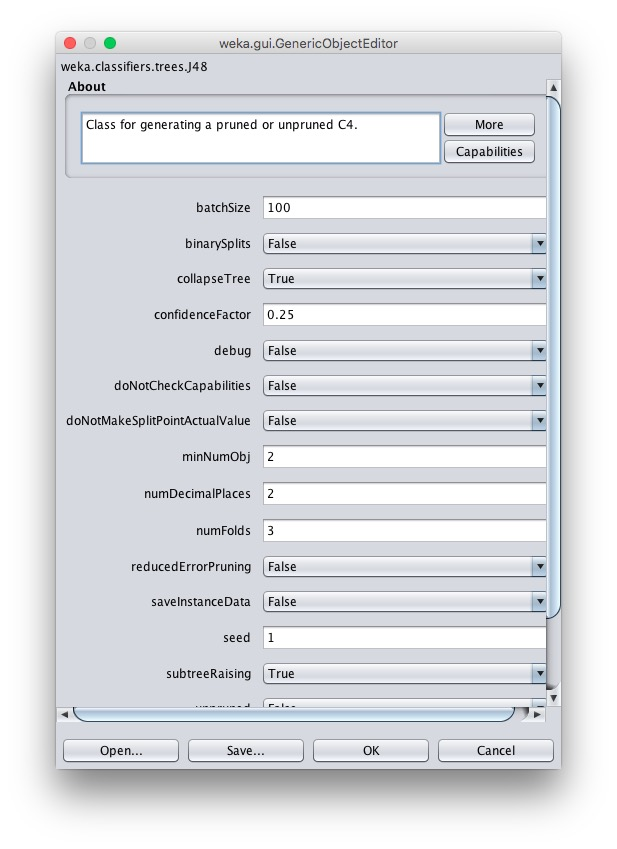
\includegraphics[scale=0.5]{tex/img/img4i.jpg}
    \caption{Configurações do Algoritmo J48}
    \label{fig:apos2}
\end{figure}

\begin{figure}[H]
    \centering
    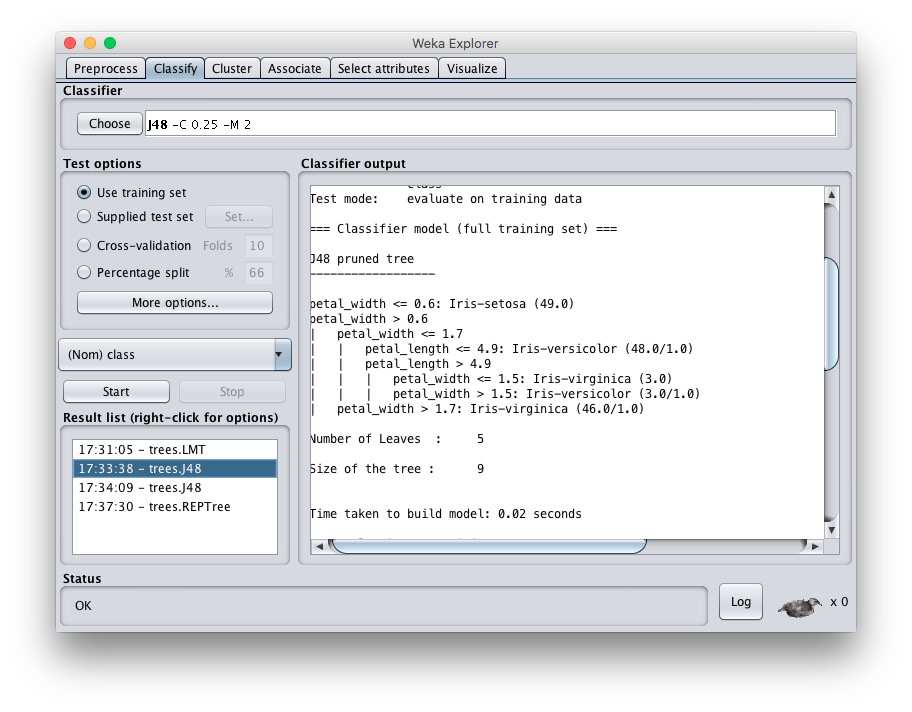
\includegraphics[scale=0.3]{tex/img/eesta.jpg}
    \caption{Algoritmo J48 usando o conjunto de treino}
    \label{fig:apos1}
\end{figure}



Foram também explorados os algoritmos LMT e REPTree mas em nenhum deles obtemos tão bons resultados como o J48, tendo em conta os erros absolutos e relativos.

\subsection{Associação}


Aplicamos também algoritmos de Associação para extrair o conhecimento a partir dos dados. O algoritmo utilizado foi o Apriori, para o qual testamos várias configurações até chegar a uma configuração ótima.

\textbf{Resultado para uma confiança maior que 60\% e suporte mínimo de 0.25}


\begin{lstlisting}[breaklines,frame=single]
Apriori
=======

Minimum support: 0.25 (37 instances)
Minimum metric <confidence>: 0.6
Number of cycles performed: 15

Generated sets of large itemsets:

Size of set of large itemsets L(1): 5

Size of set of large itemsets L(2): 1

Best rules found:

 1. petal_width='(-inf-0.34]' 40 ==> class=Iris-setosa 40    <conf:(1)> lift:(3.04) lev:(0.18) [26] conv:(26.85)
 2. class=Iris-setosa 49 ==> petal_width='(-inf-0.34]' 40    <conf:(0.82)> lift:(3.04) lev:(0.18) [26] conv:(3.58)
\end{lstlisting}


\textbf{Resultado para uma confiança maior que 60\% e suporte mínimo de 0.20}

\begin{lstlisting}[breaklines,frame=single]

Apriori
=======

Minimum support: 0.2 (30 instances)
Minimum metric <confidence>: 0.6
Number of cycles performed: 16

Generated sets of large itemsets:

Size of set of large itemsets L(1): 6

Size of set of large itemsets L(2): 3

Size of set of large itemsets L(3): 1

Best rules found:

 1. petal_width='(-inf-0.34]' 40 ==> class=Iris-setosa 40    <conf:(1)> lift:(3.04) lev:(0.18) [26] conv:(26.85)
 2. petal_length='(-inf-1.59]' 36 ==> class=Iris-setosa 36    <conf:(1)> lift:(3.04) lev:(0.16) [24] conv:(24.16)
 3. petal_length='(-inf-1.59]' petal_width='(-inf-0.34]' 32 ==> class=Iris-setosa 32    <conf:(1)> lift:(3.04) lev:(0.14) [21] conv:(21.48)
 4. petal_length='(-inf-1.59]' 36 ==> petal_width='(-inf-0.34]' 32    <conf:(0.89)> lift:(3.31) lev:(0.15) [22] conv:(5.27)
 5. petal_length='(-inf-1.59]' class=Iris-setosa 36 ==> petal_width='(-inf-0.34]' 32    <conf:(0.89)> lift:(3.31) lev:(0.15) [22] conv:(5.27)
 6. petal_length='(-inf-1.59]' 36 ==> petal_width='(-inf-0.34]' class=Iris-setosa 32    <conf:(0.89)> lift:(3.31) lev:(0.15) [22] conv:(5.27)
 7. class=Iris-setosa 49 ==> petal_width='(-inf-0.34]' 40    <conf:(0.82)> lift:(3.04) lev:(0.18) [26] conv:(3.58)
 8. petal_width='(-inf-0.34]' 40 ==> petal_length='(-inf-1.59]' 32    <conf:(0.8)> lift:(3.31) lev:(0.15) [22] conv:(3.37)
 9. petal_width='(-inf-0.34]' class=Iris-setosa 40 ==> petal_length='(-inf-1.59]' 32    <conf:(0.8)> lift:(3.31) lev:(0.15) [22] conv:(3.37)
10. petal_width='(-inf-0.34]' 40 ==> petal_length='(-inf-1.59]' class=Iris-setosa 32    <conf:(0.8)> lift:(3.31) lev:(0.15) [22] conv:(3.37)

\end{lstlisting}

Destes dados retiramos as seguintes conclusões:

\begin{itemize}
  \item Se a largura das pétalas é menor que 0.34cm então a classe da Íris é Setosa, com um grau de confiança de 100\%;
  \item Se o comprimento das pétalas é menor que 1.59cm então a classe da Íris é Setosa, com um grau de confiança de 100\%;
  \item Se o comprimento das pétalas é menor que 1.59cm e a largura das pétalas é inferior a 0.34cm então a classe da Íris é Setosa, com um grau de confiança de 100\%;
  \item Se o comprimento das pétalas é menor que 1.59cm então a largura das pétalas é também inferior a 0.34cm, com um grau de confiança de 89\%.
\end{itemize}

\subsection{Regressão Linear}

Por curiosidade experimentamos se seria possível calcular a classe da Íris a partir dos restantes parâmetros, ou seja, uma equação matemática que dado as medidas das pétalas e da sépala resultasse no tipo de Íris (1,2,3). Tínhamos a noção que parecia inviável e até um pouco confuso, o que se veio a verificar quando aplicado o modelo de Regressão Linear e por isso nada conseguimos concluir.


\begin{figure}[H]
    \centering
    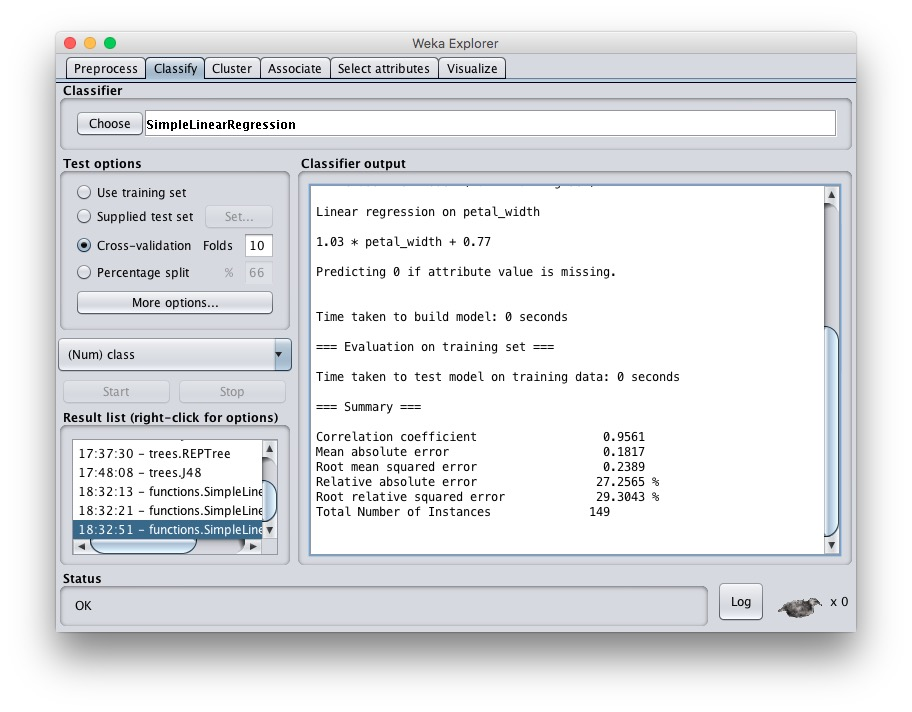
\includegraphics[scale=0.3]{tex/img/img6i.jpg}
    \caption{Regressão Linear}
    \label{fig:rl}
\end{figure}

\subsection{Resultados e Recomendações}

Conseguimos assim obter os resultados inicialmente propostos, ou seja, a partir dos dados observáveis e mensuráveis obter a classe/tipo de Íris. No entanto, os dados analisados representam apenas três tipos da flor que, segundo as nossas pesquisas, apresenta mais de 50 tipos diferentes e por isso o modelo é limitado.
De notar ainda que, os dados obtidos tanto por Associação como por Classificação são coerentes entre si.